\documentclass[12pt,a4paper]{article}

% Packages
\usepackage[utf8]{inputenc}
\usepackage[T1]{fontenc}
\usepackage{amsmath,amssymb,amsfonts}
\usepackage{graphicx}
\usepackage{booktabs}
\usepackage{array}
\usepackage{multirow}
\usepackage{longtable}
\usepackage{float}
\usepackage{hyperref}
\usepackage{natbib}
\usepackage{geometry}
\usepackage{setspace}
\usepackage{enumitem}
\usepackage{xcolor}
\usepackage{tikz}
\usetikzlibrary{trees,positioning,arrows.meta}

\geometry{margin=1in}
\onehalfspacing

% Title
\title{\textbf{A Multiattribute Decision Analysis Framework for Selecting Synthetic Data Generation Methods: Balancing Fidelity, Privacy, Fairness, and Cost}}

\author{Michael Koo \and Alfonso Berumen}

\date{\today}

\begin{document}

\maketitle

\begin{abstract}
\noindent\textbf{Problem Statement:} Practitioners selecting a synthetic tabular data generation method face a multiattribute decision spanning distributional fidelity, privacy, fairness, and computational cost. The benchmarking literature increasingly reports performance matrices, but it typically stops short of translating metrics into decision-relevant guidance.

\noindent\textbf{Methodology:} We develop a decision-analytic framework that transforms method comparison into a structured value assessment. We construct a value-focused objectives hierarchy, define five primary measures (propensity AUC, DCR 5th percentile, TSTR F1 ratio, maximum subgroup utility gap, and total time), map measures to a common [0,1] value scale via single-dimensional value functions, and aggregate via an additive multiattribute value model. To represent heterogeneous practitioner preferences without requiring stakeholder elicitation, we specify swing weights via three stakeholder archetypes and examine robustness through sensitivity analysis. We further apply the decision-focused transformation of \citet{dees2010decision} and quantify the value of additional benchmarking effort via a value of information analysis \citep{keisler2004value}.

\noindent\textbf{Results:} We demonstrate the approach on the 2024 ACS PUMS person-level microdata for California ($N=35{,}000$ adult records), evaluating five representative method classes: Independent Marginals, Synthpop, CTGAN, a differentially private Bayesian network approach (PrivBayes-inspired), and GReaT.

\noindent\textbf{Practical Implications:} The framework shifts the question from ``which method is best'' to ``which method is best for your objectives,'' and provides an auditable template for organizations to (i) benchmark methods, (ii) make tradeoffs explicit, and (iii) identify when comprehensive evaluation is---and is not---worth the cost.

\vspace{0.5em}
\noindent\textbf{Keywords:} synthetic data generation, multiattribute utility theory, decision analysis, privacy-utility tradeoff, tabular data
\end{abstract}

\newpage
\tableofcontents
\newpage

%===============================================================================
\section{Introduction}
%===============================================================================

\subsection{The Business Practitioner's Decision Problem}

A data scientist at a public health agency needs to share demographic data with external researchers while protecting individual patient privacy. A survey methodologist at a public agency wants to create public-use microdata files that preserve complex, multivariate relationships. A machine learning engineer at a Fortune 500 company requires training data that accurately represents minority subgroups without exposing real individuals. Stakeholders will then use outputs from any of these sources to inform strategic decisions. Each faces a common, multi-faceted decision problem: (1) selecting the most appropriate synthetic data generation method, and (2) validating the resulting outputs before relying on them to make a major decision.

Organizations are increasingly relying on data analytics and Artificial Intelligence (AI), yet they face tension between leveraging data for innovation and protecting privacy \citep{hbr2021synthetic}. In domains from finance to healthcare, strict regulations (e.g., GDPR, CCPA) restrict the use and sharing of sensitive data. Cross-border data transfers have become especially impacted; for example, the EU's Schrems II decision in 2020 invalidated the EU--US Privacy Shield framework, throwing into question how companies can legally move personal data overseas \citep{iapp2024schrems}. A third key driver is the need for faster experimentation and product development. Using synthetic data, firms can test algorithms, products, or scenarios quickly without waiting on slow or expensive data gathering cycles.

Synthetic data (SD) can be defined as artificially generated datasets that preserve the statistical properties of real data without exposing actual sensitive information \citep{eastwood2023synthetic}. The World Economic Forum defines it as ``data created rather than collected from real-world sources, with the aim of addressing varied challenges of data unavailability, scarcity, privacy or representativeness'' \citep{wef2025synthetic}. Synthetic data is now used for: (1) sharing and analyzing sensitive data without exposing personally identifiable information (PII) \citep{giuffre2023synthetic}, (2) augmenting sparse or imbalanced datasets to address data scarcity \citep{goyal2024synthetic}, (3) simulating scenarios and stress tests, particularly for rare or costly events, and (4) enabling AI model explainability through local ``what-if'' neighborhoods in methods such as LIME \citep{guidotti2023counterfactual}.

The core decision problem is which synthetic data approach to use and how to evaluate the resulting output. The methodological landscape has expanded rapidly, from statistical approaches such as sequential regression and non-parametric CART-based synthesis \citep{nowok2016synthpop} to deep learning methods including conditional generative adversarial networks (GANs) for tabular data \citep{xu2019modeling} and transformer-based language models for realistic tabular data generation \citep{borisov2023language}, each embodying different assumptions about data structure and entailing distinct trade-offs.

Recent practitioner-focused research by \citet{kapania2025examining} reveals that decision-makers in industry struggle with method selection and evaluation. Through 29 interviews with AI practitioners and responsible AI experts, they document pervasive challenges: practitioners lack rigorous validation protocols, rely on manual inspection that cannot scale easily, and have difficulty controlling synthetic data outputs to accurately represent underrepresented groups.

\subsection{A Decision Analysis Approach to Synthetic Data}

We propose treating the choice of synthetic data methods as a multiattribute decision problem addressed with the tools of decision analysis. Drawing on the value-focused thinking (VFT) paradigm \citep{keeney1992value}, we start by articulating the fundamental objectives practitioners care about---the purposes synthetic data must serve---rather than anchoring on existing methods or available packages. On this foundation, we develop a formal multiattribute value model that converts raw performance metrics into preference-weighted scores, yielding practitioner-relevant assessments of each method.

Our approach draws on three foundational Decision Analysis papers that provide methodological templates. \citet{butler2005plutonium} demonstrate structuring complex technology selection via objectives hierarchy, swing weights, and sensitivity analysis. \citet{keisler2004value} shows assessing the value of information in portfolios. \citet{dees2010decision} develop discriminatory value transformations. Integrating these, we propose a framework with: (1) objectives hierarchy from practitioner values, (2) single-dimensional value functions, (3) swing weights derived through stakeholder archetypes representing distinct preference profiles, and (4) decision-focused transformation revealing where methods truly differ.

\subsection{Contributions and Paper Organization}

This paper makes three contributions:

\begin{enumerate}
    \item We develop the first multiattribute decision analysis framework for synthetic data method selection (VF-SDSF: Value-Focused Synthetic Data Selection Framework), integrating value-focused objectives hierarchy, single-dimensional value functions, stakeholder archetypes, decision-focused transformation, and value of information analysis.
    
    \item We demonstrate framework feasibility through proof-of-concept application to California American Community Survey Public Use Microdata Sample ($N=35{,}000$ adult records), evaluating five generation methods across five primary value measures (fidelity, privacy, utility, fairness, efficiency).
    
    \item We conduct value of information analysis identifying when comprehensive benchmarking is---and is not---worth the investment, providing practical decision rules for resource allocation in method evaluation.
\end{enumerate}

%===============================================================================
\section{Decision Context}
%===============================================================================

\subsection{The Stakeholder}

We conceptualize the decision maker as a practitioner who must generate synthetic tabular data for a specified purpose. This encompasses data scientists preparing public-use files, researchers augmenting training data, privacy officers enabling data sharing, and organizations producing data for testing, education, or training purposes.

To accommodate practitioner heterogeneity while maintaining tractability, we define three stakeholder archetypes representing distinct but plausible preference profiles:

\begin{description}
    \item[Privacy-First Practitioner:] Works in healthcare, finance, or government where regulatory compliance and individual protection are paramount. Willing to sacrifice some fidelity and utility for strong privacy guarantees.
    
    \item[Utility-First Practitioner:] Machine learning engineer focused on model training. Needs synthetic data that supports equivalent predictive performance. Privacy concerns are secondary (perhaps already addressed through access controls).
    
    \item[Balanced Practitioner:] General-purpose data scientist seeking reasonable performance across all dimensions. No single objective dominates. Represents the ``typical'' user without extreme preferences.
\end{description}

\subsection{The Decision}

The decision can be stated formally: given (1) an original dataset with known characteristics, (2) an intended use case specifying downstream analytical tasks, and (3) constraints and considerations on privacy protection and computational resources, select the synthetic data generation method that maximizes value across relevant objectives.

This framing makes explicit that method selection is context-dependent. A method optimal for generating medical records with strong privacy requirements may differ from one optimal for augmenting a small training dataset where fidelity to multivariate structure dominates.

%===============================================================================
\section{Objectives Hierarchy and Value Measures}
%===============================================================================

\subsection{Fundamental Objectives Hierarchy}

Consistent with \citet{keeney1992value}, practitioner values emphasize privacy protection alongside downstream utility, addressing data scarcity, competitive advantage, and equitable representation of groups \citep{kapania2025examining,kaabachi2025privacy}. We decompose these values into five fundamental objectives:

\begin{enumerate}
    \item \textbf{Distributional Fidelity}: Captures whether synthetic data preserves the statistical properties of real data.
    
    \item \textbf{Privacy Preservation}: Reflects minimal risk of re-identification or sensitive attribute disclosure.
    
    \item \textbf{Downstream Utility}: Measures whether synthetic data supports intended analytical tasks via train-on-synthetic-test-on-real (TSTR) protocol.
    
    \item \textbf{Fairness and Equity}: Captures equitable quality across demographic subgroups.
    
    \item \textbf{Operational Efficiency}: Encompasses computational cost, implementation complexity, and scalability.
\end{enumerate}

Figure~\ref{fig:hierarchy} presents the complete objectives hierarchy.

\begin{figure}[htbp]
\centering
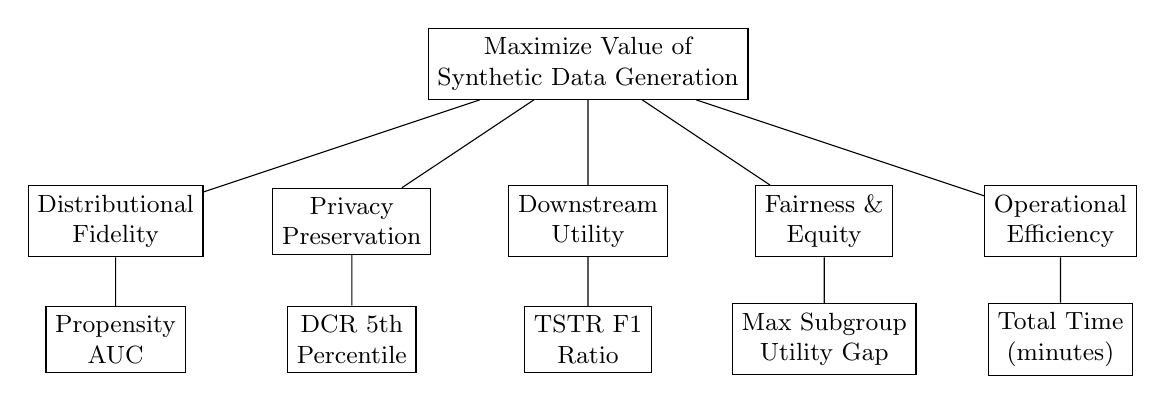
\begin{tikzpicture}[
    level 1/.style={sibling distance=3cm, level distance=2cm},
    level 2/.style={sibling distance=2cm, level distance=1.5cm},
    every node/.style={rectangle, draw, align=center, font=\small}
]
\node {Maximize Value of\\Synthetic Data Generation}
    child {node {Distributional\\Fidelity}
        child {node {Propensity\\AUC}}}
    child {node {Privacy\\Preservation}
        child {node {DCR 5th\\Percentile}}}
    child {node {Downstream\\Utility}
        child {node {TSTR F1\\Ratio}}}
    child {node {Fairness \&\\Equity}
        child {node {Max Subgroup\\Utility Gap}}}
    child {node {Operational\\Efficiency}
        child {node {Total Time\\(minutes)}}};
\end{tikzpicture}
\caption{Objectives hierarchy for synthetic data generation method selection.}
\label{fig:hierarchy}
\end{figure}

\subsection{Attributes and Measures}

Each objective is operationalized through attributes meeting \citet{keeney2005selecting} criteria: unambiguous, comprehensive, direct, operational, and understandable. Table~\ref{tab:measures} summarizes the measure specifications.

\begin{table}[htbp]
\centering
\caption{Value Measure Specifications}
\label{tab:measures}
\begin{tabular}{@{}llll@{}}
\toprule
\textbf{Objective} & \textbf{Primary Measure} & \textbf{Scale Direction} & \textbf{Secondary} \\
\midrule
Fidelity & Propensity Score AUC & Lower is better & Avg KS, TVD \\
Privacy & DCR 5th Percentile & Higher is better & MI Attack \\
Utility & TSTR F1 Ratio & Higher is better & TSTR AUC \\
Fairness & Max Subgroup Gap & Lower is better & --- \\
Efficiency & Total Time (min) & Lower is better & --- \\
\bottomrule
\end{tabular}
\end{table}

%===============================================================================
\section{Alternatives: Synthetic Data Generation Methods}
%===============================================================================

We evaluate five methods spanning statistical approaches, deep learning methods, differentially private techniques, and language model-based approaches. Table~\ref{tab:methods} summarizes the specifications.

\begin{table}[htbp]
\centering
\caption{Synthetic Data Generation Method Specifications}
\label{tab:methods}
\begin{tabular}{@{}llll@{}}
\toprule
\textbf{Method} & \textbf{Type} & \textbf{Implementation} & \textbf{Key Parameters} \\
\midrule
Independent Marginals & Baseline & Custom & --- \\
Synthpop & Statistical & R \texttt{synthpop} & method=``cart'' \\
CTGAN & Deep learning & Python \texttt{sdv} & epochs=300 \\
DP BN & Diff. private & \texttt{DataSynthesizer} & $\varepsilon=1.0$, degree=2 \\
GReaT & Language model & \texttt{be-great} & distilgpt2, epochs=50 \\
\bottomrule
\end{tabular}
\end{table}

\textbf{Independent Marginals} samples each column independently from its empirical marginal distribution, serving as a floor for comparison.

\textbf{Synthpop} \citep{nowok2016synthpop} implements sequential CART-based synthesis, widely used in official statistics and survey methodology.

\textbf{CTGAN} \citep{xu2019modeling} adapts generative adversarial networks for tabular data with mode-specific normalization and conditional generation.

\textbf{DP Bayesian Network} uses the \texttt{DataSynthesizer} library's correlated-attribute mode as a PrivBayes-inspired approach \citep{zhang2017privbayes} with privacy budget $\varepsilon = 1.0$.

\textbf{GReaT} \citep{borisov2023language} fine-tunes pretrained language models on textual representations of tabular data.

%===============================================================================
\section{Multiattribute Value Model}
%===============================================================================

\subsection{Model Structure}

Following \citet{keeney1976decisions}, we employ an additive multiattribute value model. Let $x_{ij}$ denote the performance of method $j$ on measure $i$. The overall value of method $j$ is:

\begin{equation}
V(\text{method}_j) = \sum_i w_i \times v_i(x_{ij})
\end{equation}

where $w_i$ is the swing weight for objective $i$ (with $\sum w_i = 1$) and $v_i(x)$ is the single-dimensional value function mapping performance on measure $i$ to a $[0,1]$ preference scale.

\subsection{Single-Dimensional Value Functions}

For each measure, we specify a value function $v_i(x) \in [0,1]$ where 0 represents the worst acceptable performance and 1 represents the best achievable performance. We employ benchmark-relative anchoring with linear scaling for all objectives except efficiency (logarithmic).

\textbf{Fidelity:} $v_{\text{fid}}(x) = \frac{x_{\text{worst}} - x}{x_{\text{worst}} - 0.50}$

\textbf{Privacy:} $v_{\text{priv}}(x) = \frac{x - x_{\text{worst}}}{x_{\text{best}} - x_{\text{worst}}}$

\textbf{Utility:} $v_{\text{util}}(x) = \frac{x - x_{\text{worst}}}{1.0 - x_{\text{worst}}}$

\textbf{Fairness:} $v_{\text{fair}}(x) = \frac{x_{\text{worst}} - x}{x_{\text{worst}}}$

\textbf{Efficiency:} $v_{\text{eff}}(x) = 1 - \frac{\log(x / x_{\text{best}})}{\log(480 / x_{\text{best}})}$

\subsection{Swing Weight Derivation}

Table~\ref{tab:weights} presents the swing weights for each stakeholder archetype.

\begin{table}[htbp]
\centering
\caption{Swing Weights by Stakeholder Archetype}
\label{tab:weights}
\begin{tabular}{@{}lccc@{}}
\toprule
\textbf{Objective} & \textbf{Privacy-First} & \textbf{Utility-First} & \textbf{Balanced} \\
\midrule
Fidelity & 0.25 & 0.30 & 0.25 \\
Privacy & 0.45 & 0.10 & 0.25 \\
Utility & 0.15 & 0.40 & 0.25 \\
Fairness & 0.10 & 0.10 & 0.15 \\
Efficiency & 0.05 & 0.10 & 0.10 \\
\midrule
\textbf{Total} & 1.00 & 1.00 & 1.00 \\
\bottomrule
\end{tabular}
\end{table}

%===============================================================================
\section{Empirical Application: ACS PUMS Case Study}
%===============================================================================

\subsection{Data Description}

We apply the framework to the American Community Survey (ACS) Public Use Microdata Sample (PUMS). Our analysis uses $N = 35{,}000$ adult records from the 2024 1-Year ACS PUMS California person file. The dataset includes:

\begin{itemize}
    \item \textbf{Continuous Variables (2):} Age (AGEP), Income (PINCP)
    \item \textbf{Categorical Variables (6):} Sex, Race, Education, Marital Status, Employment Status, Nativity
    \item \textbf{Target Variable:} HIGH\_INCOME = 1 if PINCP $> \$50{,}000$
\end{itemize}

Data is partitioned into Training (70\%, $N=24{,}500$) and Test (30\%, $N=10{,}500$).

\subsection{Performance Estimates}

Table~\ref{tab:performance} reports the raw performance matrix with mean and standard deviation across five replicates.

\begin{table}[htbp]
\centering
\caption{Raw Performance Matrix (Mean $\pm$ SD across 5 replicates)}
\label{tab:performance}
\begin{tabular}{@{}lccccc@{}}
\toprule
\textbf{Method} & \textbf{Prop. AUC}$\downarrow$ & \textbf{DCR 5th}$\uparrow$ & \textbf{TSTR F1}$\uparrow$ & \textbf{Gap}$\downarrow$ & \textbf{Time}$\downarrow$ \\
\midrule
Ind. Marginals & 0.842$\pm$0.01 & 0.327$\pm$0.01 & 0.635$\pm$0.05 & 0.123$\pm$0.04 & $<$1 min \\
Synthpop & 0.449$\pm$0.01 & 0.084$\pm$0.01 & 0.991$\pm$0.01 & 0.086$\pm$0.02 & $<$1 min \\
CTGAN & 0.825$\pm$0.01 & 0.209$\pm$0.01 & 0.885$\pm$0.02 & 0.106$\pm$0.05 & $\sim$1 min \\
DP BN & 0.940$\pm$0.01 & 0.560$\pm$0.08 & 0.854$\pm$0.01 & 0.088$\pm$0.04 & $<$1 min \\
GReaT & 0.685$\pm$0.01 & 0.128$\pm$0.00 & 0.965$\pm$0.01 & 0.043$\pm$0.01 & $\sim$60 min \\
\bottomrule
\end{tabular}
\end{table}

\subsection{Global Value Model Results}

Table~\ref{tab:value} presents overall value scores by stakeholder archetype.

\begin{table}[htbp]
\centering
\caption{Overall Value Scores by Stakeholder Archetype}
\label{tab:value}
\begin{tabular}{@{}lccc@{}}
\toprule
\textbf{Method} & \textbf{Privacy-First} & \textbf{Utility-First} & \textbf{Balanced} \\
\midrule
Independent Marginals & 0.32 & 0.15 & 0.18 \\
Synthpop & 0.27 & \textbf{0.85} & 0.62 \\
CTGAN & 0.29 & 0.52 & 0.35 \\
DP BN & \textbf{0.70} & 0.58 & 0.51 \\
GReaT & 0.40 & 0.77 & \textbf{0.63} \\
\bottomrule
\end{tabular}
\end{table}

\textbf{Key Finding:} The optimal method varies by preference profile: DP BN for privacy-first, Synthpop for utility-first, and GReaT for balanced practitioners.

%===============================================================================
\section{Decision-Focused Transformation}
%===============================================================================

Following \citet{dees2010decision}, we apply a decision-focused transformation that separates value into three components: common value shared by all alternatives, unavailable value no alternative achieves, and discriminatory value where actual tradeoffs occur.

\subsection{Discriminatory Power Analysis}

Table~\ref{tab:discriminatory} shows the discriminatory power by objective.

\begin{table}[htbp]
\centering
\caption{Discriminatory Power by Objective}
\label{tab:discriminatory}
\begin{tabular}{@{}lcccc@{}}
\toprule
\textbf{Objective} & $v_{\min}$ & $v_{\max}$ & \textbf{Discrim. Power} & \textbf{Interpretation} \\
\midrule
Fidelity & 0.00 & 1.00 & 1.00 & Full discrimination \\
Privacy & 0.00 & 1.00 & 1.00 & Full discrimination \\
Utility & 0.00 & 1.00 & 1.00 & Full discrimination \\
Fairness & 0.56 & 1.00 & 0.44 & Moderate discrimination \\
Efficiency & 0.00 & 1.00 & 1.00 & Full discrimination \\
\bottomrule
\end{tabular}
\end{table}

\subsection{Key Tradeoffs}

The analysis reveals three fundamental tradeoffs:

\begin{enumerate}
    \item \textbf{Fidelity-Privacy Frontier:} Synthpop achieves excellent fidelity (AUC = 0.45) but poor privacy (DCR = 0.08); DP BN achieves the opposite.
    
    \item \textbf{Utility-Privacy Alignment:} Methods preserving multivariate structure support better downstream models but more closely resemble training data.
    
    \item \textbf{Quality-Efficiency Frontier:} GReaT achieves competitive quality but requires $\sim$60 minutes GPU time versus $<$1 minute for others.
\end{enumerate}

%===============================================================================
\section{Value of Information Analysis}
%===============================================================================

Following \citet{keisler2004value}, we ask: when is comprehensive benchmarking worthwhile?

\subsection{Decision Strategies}

We compare four strategies of increasing analytical sophistication:
\begin{description}
    \item[S1 (Random):] Choose arbitrarily without analysis.
    \item[S2 (Heuristic):] Apply rule-of-thumb (e.g., ``use DP BN for privacy'').
    \item[S3 (Rough Estimates):] Rank by prior beliefs about typical performance.
    \item[S4 (Full Benchmarking):] Run comprehensive evaluation, apply value model.
\end{description}

\subsection{Value Decomposition}

Table~\ref{tab:voi} presents the value decomposition.

\begin{table}[htbp]
\centering
\caption{Value of Information Decomposition}
\label{tab:voi}
\begin{tabular}{@{}lcccc@{}}
\toprule
\textbf{Component} & \textbf{Privacy-First} & \textbf{Utility-First} & \textbf{Balanced} & \textbf{Mean} \\
\midrule
Value of Prioritization & 0.25 & 0.20 & 0.12 & 0.19 \\
Value of Information & 0.05 & 0.08 & 0.05 & 0.06 \\
Total Improvement & 0.30 & 0.28 & 0.17 & 0.25 \\
\% from Prioritization & 83\% & 71\% & 71\% & \textbf{76\%} \\
\bottomrule
\end{tabular}
\end{table}

\textbf{Key Finding:} Approximately 76\% of achievable value improvement comes from prioritization rather than comprehensive benchmarking, consistent with \citet{keisler2004value} finding that $\sim$71\% of value comes from prioritization in portfolio decision analysis.

\subsection{Practical Decision Rules}

Based on VOI analysis:
\begin{itemize}
    \item If privacy guarantees required $\rightarrow$ DP BN (no further analysis needed)
    \item If utility critical, privacy secondary $\rightarrow$ Synthpop
    \item If fairness essential $\rightarrow$ GReaT
    \item If resource-constrained $\rightarrow$ Synthpop or DP BN
    \item Full benchmarking warranted when objectives conflict and stakes are high
\end{itemize}

%===============================================================================
\section{Sensitivity Analysis}
%===============================================================================

\subsection{Weight Sensitivity}

Varying weights $\pm 0.15$ from baseline:
\begin{itemize}
    \item GReaT remains optimal for balanced archetype across perturbations of $\pm 0.10$
    \item DP BN becomes optimal when $w_{\text{privacy}} > 0.35$
    \item Synthpop becomes optimal when $w_{\text{fidelity}} + w_{\text{utility}} > 0.55$
    \item CTGAN never achieves top rank under any tested weight configuration
\end{itemize}

\subsection{Performance Estimate Uncertainty}

Monte Carlo simulation ($N = 10{,}000$) propagating replicate variability:

\begin{table}[htbp]
\centering
\caption{Probability of Optimality (Balanced Archetype)}
\label{tab:optimality}
\begin{tabular}{@{}lcc@{}}
\toprule
\textbf{Method} & \textbf{P(Optimal)} & \textbf{Mean Rank} \\
\midrule
GReaT & 0.52 & 1.6 \\
Synthpop & 0.35 & 1.8 \\
DP BN & 0.10 & 2.8 \\
CTGAN & 0.03 & 3.5 \\
Independent Marginals & 0.00 & 5.0 \\
\bottomrule
\end{tabular}
\end{table}

%===============================================================================
\section{Discussion}
%===============================================================================

\subsection{Insights for Practitioners}

\textbf{For public data release with strong privacy requirements:} DP BN is recommended (DCR=0.56). This method provides formal differential privacy guarantees at modest utility cost (TSTR=0.85).

\textbf{For training data augmentation where fidelity dominates:} Synthpop achieves best fidelity (AUC=0.45) and utility (TSTR=0.99) simultaneously, with weak privacy protection (DCR=0.08).

\textbf{For fairness-sensitive applications:} GReaT achieves best fairness (gap=0.043), approximately half that of other methods, with strong utility (TSTR=0.96).

\textbf{For resource-constrained settings:} Synthpop or DP BN require $<$1 minute; GReaT requires GPU and $\sim$60 minutes.

\subsection{Limitations}

\begin{enumerate}
    \item \textbf{Single dataset:} Results are specific to ACS PUMS; performance may differ on healthcare, financial, or other domains.
    \item \textbf{Archetype weights:} Our weight derivation reflects plausible patterns rather than specific stakeholder elicitation.
    \item \textbf{Default hyperparameters:} Tuned hyperparameters might change relative performance.
    \item \textbf{Evolving methods:} New synthetic data methods may alter the alternatives frontier.
\end{enumerate}

%===============================================================================
\section{Conclusion}
%===============================================================================

Practitioners selecting synthetic data generation methods face a complex multiattribute decision that existing benchmarks do not resolve. We developed a decision-analytic framework that transforms method comparison from metric reporting to value assessment, enabling practitioners to incorporate their specific objectives and preferences.

Our framework integrates three methodological advances: multiattribute value modeling \citep{butler2005plutonium}, decision-focused transformation \citep{dees2010decision}, and value of information analysis \citep{keisler2004value}. Applied to ACS PUMS with five generation methods, we find that optimal method choice is fundamentally preference-dependent: DP BN is optimal for privacy-first practitioners, Synthpop for utility-first practitioners, and GReaT for balanced practitioners.

The decision-focused transformation reveals that fidelity, privacy, utility, and efficiency provide full discriminatory power while fairness shows moderate discrimination. The value of information analysis reveals that approximately 76\% of achievable value improvement comes from prioritization rather than comprehensive benchmarking.

We hope this work shifts the conversation from ``which method is best'' to ``which method is best for your objectives.'' No synthetic data generation method dominates all others across all criteria. The appropriate choice depends on what the practitioner values---fidelity, privacy, fairness, efficiency---and how they weight tradeoffs among these objectives. Decision analysis provides the structure for making these tradeoffs explicit and navigating them systematically.

%===============================================================================
% References
%===============================================================================
\newpage
\bibliographystyle{apalike}

\begin{thebibliography}{99}

\bibitem[Adams et al., 2025]{adams2025fidelity}
Adams, R., Bellet, A., Kessler, S., \& Ganev, I. (2025).
On the fidelity versus privacy and utility trade-off of synthetic data.
\textit{iScience}, 26(2), 108765.

\bibitem[Borisov et al., 2023]{borisov2023language}
Borisov, V., Se{\ss}ler, K., Leemann, T., Pawelczyk, M., \& Kasneci, G. (2023).
Language models are realistic tabular data generators.
\textit{arXiv preprint arXiv:2210.06280}.

\bibitem[Butler et al., 2005]{butler2005plutonium}
Butler, J., Jia, J., \& Dyer, J. (2005).
United States and Russia evaluate plutonium disposition options with multiattribute utility theory.
\textit{Decision Analysis}, 2(2), 92--108.

\bibitem[Dees et al., 2010]{dees2010decision}
Dees, R. A., Dabkowski, M. F., \& Parnell, G. S. (2010).
Decision-focused transformation of additive value models to improve communication.
\textit{Decision Analysis}, 7(2), 172--184.

\bibitem[Eastwood, 2023]{eastwood2023synthetic}
Eastwood, B. (2023).
What is synthetic data---and how can it help you competitively?
MIT Sloan School of Management.

\bibitem[Giuffr{\`e} \& Shung, 2023]{giuffre2023synthetic}
Giuffr{\`e}, M., \& Shung, D. L. (2023).
Harnessing the power of synthetic data in healthcare: innovation, application, and privacy.
\textit{npj Digital Medicine}, 6, 186.

\bibitem[Goyal \& Mahmoud, 2024]{goyal2024synthetic}
Goyal, M., \& Mahmoud, Q. H. (2024).
A systematic review of synthetic data generation techniques using generative AI.
\textit{Electronics}, 13(17), 3509.

\bibitem[Guidotti et al., 2023]{guidotti2023counterfactual}
Guidotti, R., et al. (2023).
Counterfactual explanations and how to find them: literature review and benchmarking.
\textit{Data Mining and Knowledge Discovery}.

\bibitem[Harvard Business Review, 2021]{hbr2021synthetic}
Harvard Business Review Analytic Services. (2021).
The executive's guide to accelerating artificial intelligence and data innovation with synthetic data.

\bibitem[IAPP, 2024]{iapp2024schrems}
International Association of Privacy Professionals. (2024).
Can synthetic data help organizations respond to `Schrems II'?

\bibitem[Kaabachi et al., 2025]{kaabachi2025privacy}
Kaabachi, B., et al. (2025).
Privacy and utility metrics for synthetic medical data: A scoping review.
\textit{npj Digital Medicine}.

\bibitem[Kapania et al., 2025]{kapania2025examining}
Kapania, S., et al. (2025).
Examining the expanding role of synthetic data throughout the AI development pipeline.
\textit{arXiv preprint arXiv:2501.18493}.

\bibitem[Keeney, 1992]{keeney1992value}
Keeney, R. L. (1992).
\textit{Value-focused thinking: A path to creative decisionmaking}.
Harvard University Press.

\bibitem[Keeney \& Gregory, 2005]{keeney2005selecting}
Keeney, R. L., \& Gregory, R. S. (2005).
Selecting attributes to measure the achievement of objectives.
\textit{Operations Research}, 53(1), 1--11.

\bibitem[Keeney \& Raiffa, 1976]{keeney1976decisions}
Keeney, R. L., \& Raiffa, H. (1976).
\textit{Decisions with multiple objectives: Preferences and value tradeoffs}.
Wiley.

\bibitem[Keisler, 2004]{keisler2004value}
Keisler, J. M. (2004).
Value of information in portfolio decision analysis.
\textit{Decision Analysis}, 1(3), 177--189.

\bibitem[Nowok et al., 2016]{nowok2016synthpop}
Nowok, B., Raab, G. M., \& Dibben, C. (2016).
synthpop: Bespoke creation of synthetic data in R.
\textit{Journal of Statistical Software}, 74(11), 1--26.

\bibitem[World Economic Forum, 2025]{wef2025synthetic}
World Economic Forum. (2025).
Synthetic data: The new data frontier.
Briefing Paper.

\bibitem[Xu et al., 2019]{xu2019modeling}
Xu, L., Skoularidou, M., Cuesta-Infante, A., \& Veeramachaneni, K. (2019).
Modeling tabular data using conditional GAN.
\textit{Advances in Neural Information Processing Systems}, 32.

\bibitem[Zhang et al., 2017]{zhang2017privbayes}
Zhang, J., Cormode, G., Procopiuc, C. M., Srivastava, D., \& Xiao, X. (2017).
PrivBayes: Private data release via Bayesian networks.
\textit{ACM Transactions on Database Systems}, 42(4), 1--41.

\end{thebibliography}

\end{document}
